\chapter{Background}\label{chap:background}


\section{Student engagement and interaction}
\todo{Performance, Læringsutbytte, Studenters motivasjon...}
While one may expect that attending class will have a positive effect on a student's academic performance, Stefan Büchele \cite{Buchele2021} has found that simply attending class has a low correlation with performance. What affects performance more is how the attendance is experienced by the students, or rather their level of engagement when attending class. Engagement can be seen as consisting of three parts as exlained by Lei et al. \cite{lei2018}. Behavioural engangement is the level of involvement in learning activities. Cognitive engagement is the level of cognitive effort and self-regulation when in a learning environment. Emotional engagement is how strongly students react to their learning environment, ranging from their interest, emotions and sense of belonging.

Büchele \cite{Buchele2021} finds that behavioural engagement fully mediates performance, in the sense that having the students perform some action contributes to making attendance positively affect their performance. Tutorial sessions tend to have a greater impact on the students' performance than do normal lectures, which Büchele argues is due to tutorials providing students with more behavioural engagement and that students more often tend to be passive listeners in normal lectures. Cognitive engagement was also shown to mediate performance, but too weakly for the result to be conclusive. He goes on to propose more use of flipped classroom or response systems in normal lectures, as these are shown to help engagement, especially in large classes. Lei et al. \cite{lei2018} have, through a meta-analysis of 69 studies, found that all three levels of engagement positively correlate with academic performance, though they are careful with stating any causation. Behavioural engagement has the strongest correlation, then cognitive and lastly emotional engagement. They also support the argument that especially behavioural engagement creates a sort of virtuous cycle, where engagement leads to better academic performance, which goes on to motivate the student to engage more, which again improves their performance. 

In terms of student-instructor interaction, Flodén \cite{floden2017} has found that feedback is important, with most instructors regarding feedback from students as positive and useful for helping them improve and adapt their teaching. Flodén also noted that, in their feedback, students tend to want more tutorials, seminars and case studies. This goes to show that students prefer learning environments that faciliates more engagement. However, in comparison to normal lectures, these are more expensive ways of teaching, requiring a higher budget and more resources. Cost, therefore, seems to be a hinderance even when both students and instructor would prefer more engaging teaching formats.
\todo{Still needs something about student-teacher interaction and motivation}


% Interaction and engagement between students and teachers in the classroom is widely perceived as one of the most important factors in learning outcomes, academic performance and general motivation [src]. Additionally, high levels of interaction and engagement often correlate [src] with improved understanding, retention and ability to use the knowledge in other areas. A potential reason to why this happens is that the increased engagement can potentially make learners more connected with the materials. 

% Achieving high levels of interactions and engagement can be difficult and resource intensive. In smaller classes, the teacher can often use methods like direct dialogue to communicate and let everyone actively participate throgh questions and discussions. While this is a perfectly good solution, it does not scale well for larger classes. In large classes there is simply not enough time or resources to ensure that every student can contribute one a one-to-one basis. This often leads to a more passive teaching environment [src] with less interaction. This can cause a missed opportunity for effective learning. 

% To mitigate these issues, educational technologies like student response systems have been introduced. These systems aims to facilitate direct participation in a classroom through various technology, often through asking real-time questions. One of the main benefits of these digital systems is that the logistical issues of large classes are no longer present. In the following section we will go in more detail through the previous and current solution, and mention benefits and issues with these technologies regarding interaction and learning outcomes. 

\begin{comment}
    Attendance alone has a low correlation with performance
    Important how the attendence is experienced
    Cognitive engagement partially mediates performance
    Behavourial engagement fully mediates performance
    Tutorials more so than normal lectures
    Flipped classroom and response systems are shown to help engagement in large classes
\cite{Buchele2021}

    
    Challenges:
        Hard to get "just-in-time" feedback from students
        Limited time providing individual feedback
        Limited peer interaction and instructor-learner interaction
        High affective filter when voicing personal views in class
    Benefits:
        Anonymous responses -> Less affective filter, more confident
        Everyone's voice is heard, no one gets to dominate discussion
    Students responded positively to the introduction of a response system
        Great fun, Instantaneous feedback, participation, interaction, independent thinking

    - Bloom’s taxonomy
    - Remember, Understand, Apply → True/False, Multiple-choice
        - Stimulate factual recall
    - Analyse, Evaluate, Create → Item-ranking, open-ended, word-cloud
        - Elicite opinions and views, reveal or challenge misconceptions on a topic

    Word cloud > Brief answers or comments > Item ranking > Multiple-choice
\cite{shi2023}
\end{comment}


\section{Open-ended questions in education}
\todo{Effect of open-ended questions: reflection, critical thinking, bearbeide kunnskap}
Bloom's taxonomy \cite{bloom1964taxonomy} is an often used tool to explain studentsæ different levels of thinking. It uses six different categories ranging from simple recall of facts to higher level thinking. The categories are knowledge, comprehension, application, analysis, synthesis and evaluation.
\todo{Still haven't found anything :(}


% \subsection{Live-questions (traditional)}
% % not worth mentioning?
% % Can be raise-of-hands as well? 

% We have mostly focused on digital solutions, but it can be nice to get an overview of non-digital alternatives.

% Raise-of-hands allow the lecturer to ask a question and cast a vote. This can either be yes/no, multiple-choice questions. While this is easy to implement, getting exact measures of distributions might be difficult. In digital classrooms, it might be difficult to get an overview if respondends have low camera quality or poor connection. In large lecture halls it might not be possible to see everyone present from the perspective of the lecturer.



\section{Response systems}\label{sec:responsesystems}
% https://tophat.com/blog/classroom-clickers/
Student response systems go by many names, such as classroom response systems, audience response systems, polling systems, clickers and electronic voting systems. However, in this report we will refer to them simply as ``response systems''. These systems are a form of interactive technology used to increase interaction between a presenter and the audience, mainly though allowing the audience to respond to the presenter's questions in real-time without the need for hand-raising or answering aloud. In the context of education, the presenter is the instructor and the audience is the students. Their history runs back to the 1970s, with their introduction in the education sphere starting in the 1990s. \cite{resyslitrev}

\subsection{Clickers}
Traditional clickers used in classrooms consist of a combination of hardware and software with the aim of increasing engagement and interactivity. The hardware is typically a combination of remote-controlled devices - similar to a TV-remote using infra-red or radio signals - and a receiver that can collect input from the remotes and aggregate the inputs \cite{shi2023}. An illustration of a clicker system can be seen in figure \ref{fig:clickersetup}. It usually works by the teacher asking a multiple-choice question to the class, and then each individual can send in the answer through these devices. The teacher will usually be able to see the results and can share them with the class. For instance, a digital dashboard solution can automatically create graphs and visualisations of how the students have answered. 

\begin{figure}[h!]
    \centering
    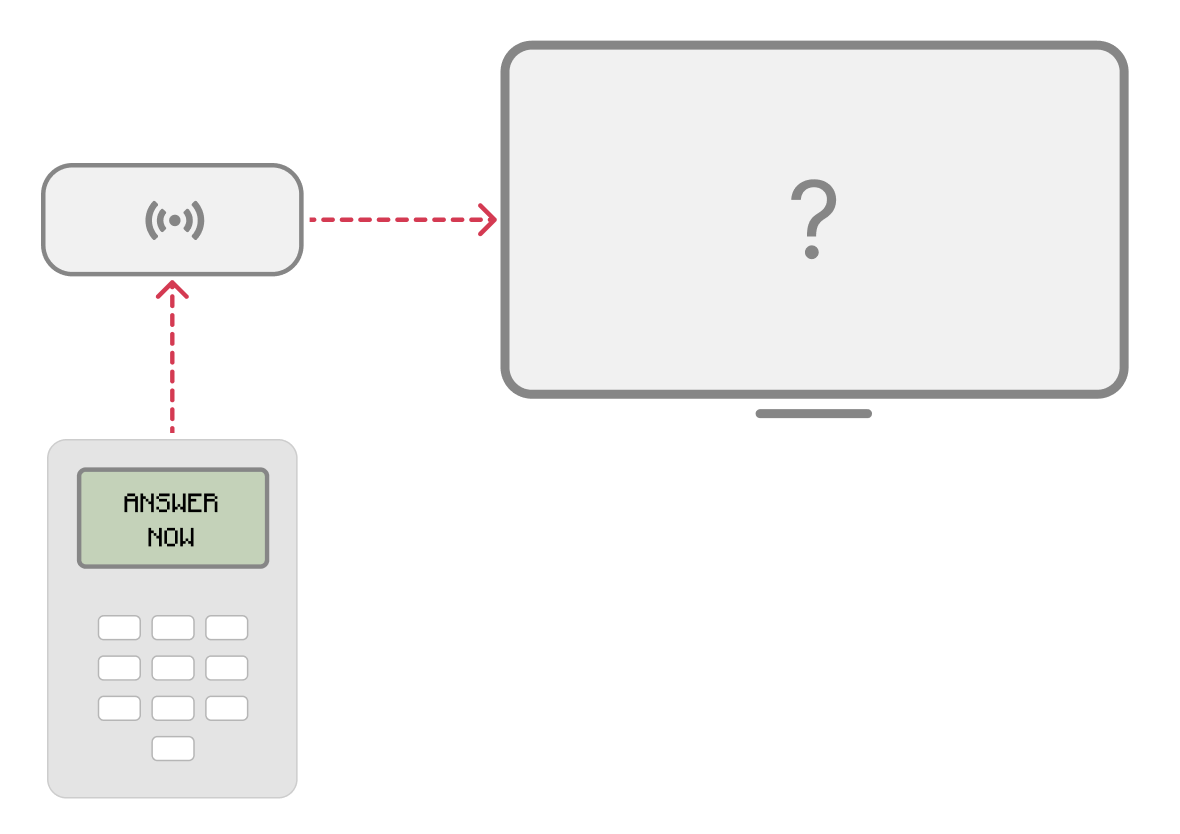
\includegraphics[width=.8\linewidth]{figures/clickers-illustration.png}
    \caption{A typical classroom setup with clickers, a receiver and a display screen}
    \label{fig:clickersetup}
\end{figure}

Compared to raising hands to answer questions or cast votes in the classroom, traditional clickers facilitates student-instructor interaction to a greater extent by allowing students to respond anonymously and providing instantaneous visualisations of the answers that can be acted upon. This also makes it possible for instructors to monitor students' understanding and misconceptions in large classrooms \cite{hunsu2016}. However, compared to more modern web-based response systems, traditional clickers are both more costly due to the need for dedicated hardware and more limited in that they only allow multiple-choice responses \cite{resyslitrev}. It is, additionally, hard to provide students with feedback on whether their responses have been registered or not and to track responses across multiple questions to implement features such as scores. This is because the remote-controlled devices do not have a graphical user interface and the signal only goes on way, from the devices to the receiver system.

\subsection{Web-based response systems}
Nowadays, web-based response systems have mostly replaced traditional clickers. These systems communicate over the internet, or in some cases over bluetooth, and can run in the a browser or as an app, which allows students to use their own mobile device, be that a smartphone, tablet or laptop \cite{resyslitrev}. This drives down the cost as hardware does not need to be acquired; it is usually enough to buy a licence from the vendor of the response system. Communication over the internet also comes with other advantages. Students can interact with the instructor and the rest of the class even when not being physically present in the classroom, making digital classrooms and MOOCs more engaging. It also allows for much more flexibility in how students use and engage with the system \cite{resyslitrev}. Instead of a controller with some buttons, the students are now met with a graphical interface. This way the students can receive more personalised feedback and elements of gamification can be added. The system is no longer restricted to multiple-choice questions anymore. An array of different question types are now featured in response systems, such as scales, item-ranking, word-clouds, and various forms of open-text responses.

Kocak \cite{resyslitrev} has, through a systematic literature review on web-based response systems, found that response systems help fend off boredom during class. This is achieved through creating a more active and joyful learning environment, where students' are encouraged to actively participate in answering questions or solving tasks. Response systems make students find the classes more interesting, and by better maintaining their concentration and providing them with insight into what types of questions and tasks they may encounter in the future, response systems also help reduce anxiety and stress. The systems help instructors and students alike to discover knowledge-gaps through testing the students knowledge and through direct feedback submitted by students. Students are also informed of what their peers think and know in this way. Lastly, Kocak found that the ability to respond anynously is crucial for the students' willingness to participate actively. 

Currently, lecturers at NTNU have access to mainly two response systems, Mentimeter and Kahoot!. These two systems will, therefore, be relevant for the collection of open-text responses in our master's thesis and for comparison when evaluating the system. We present them subsequently.

\subsection{Mentimeter}
Mentimeter describes itelf as an audience engagement platform \cite{mentimeterAudienceResponse}. Mentimeter works by presenting slides to an audience, be that in a classroom, board meeting or at a conference. The system runs in a browser, and the audience can join from their own devices by inputing the presentation's pin on the Mentimeter website or scanning the QR-code. A slide can either feature mutlimedia content, a type of quiz competition, or an interactive question. The audience responses will be shown on the slides in real-time, providing both the instructor and the students with quick feedback and insights. Mentimeter offers many types of interactive questions, such as multiple choice, Q\&A and ranking. For this project and for the master's thesis, we are only interested in the question type ``Open Ended'', which asks a question and lets the audience enter open-text responses of up to 200 characters per response. Mentimeter can collect responses anonymously out-of-the-box. An example of a slide with an open-ended question and open-text responses is shown in figure \ref{fig:mentimeterscreenshots} as displayed on a screen for the whole class and as seen by students on their smartphones.

\begin{figure}[h!]
\centering
\begin{subfigure}{0.65\textwidth}
    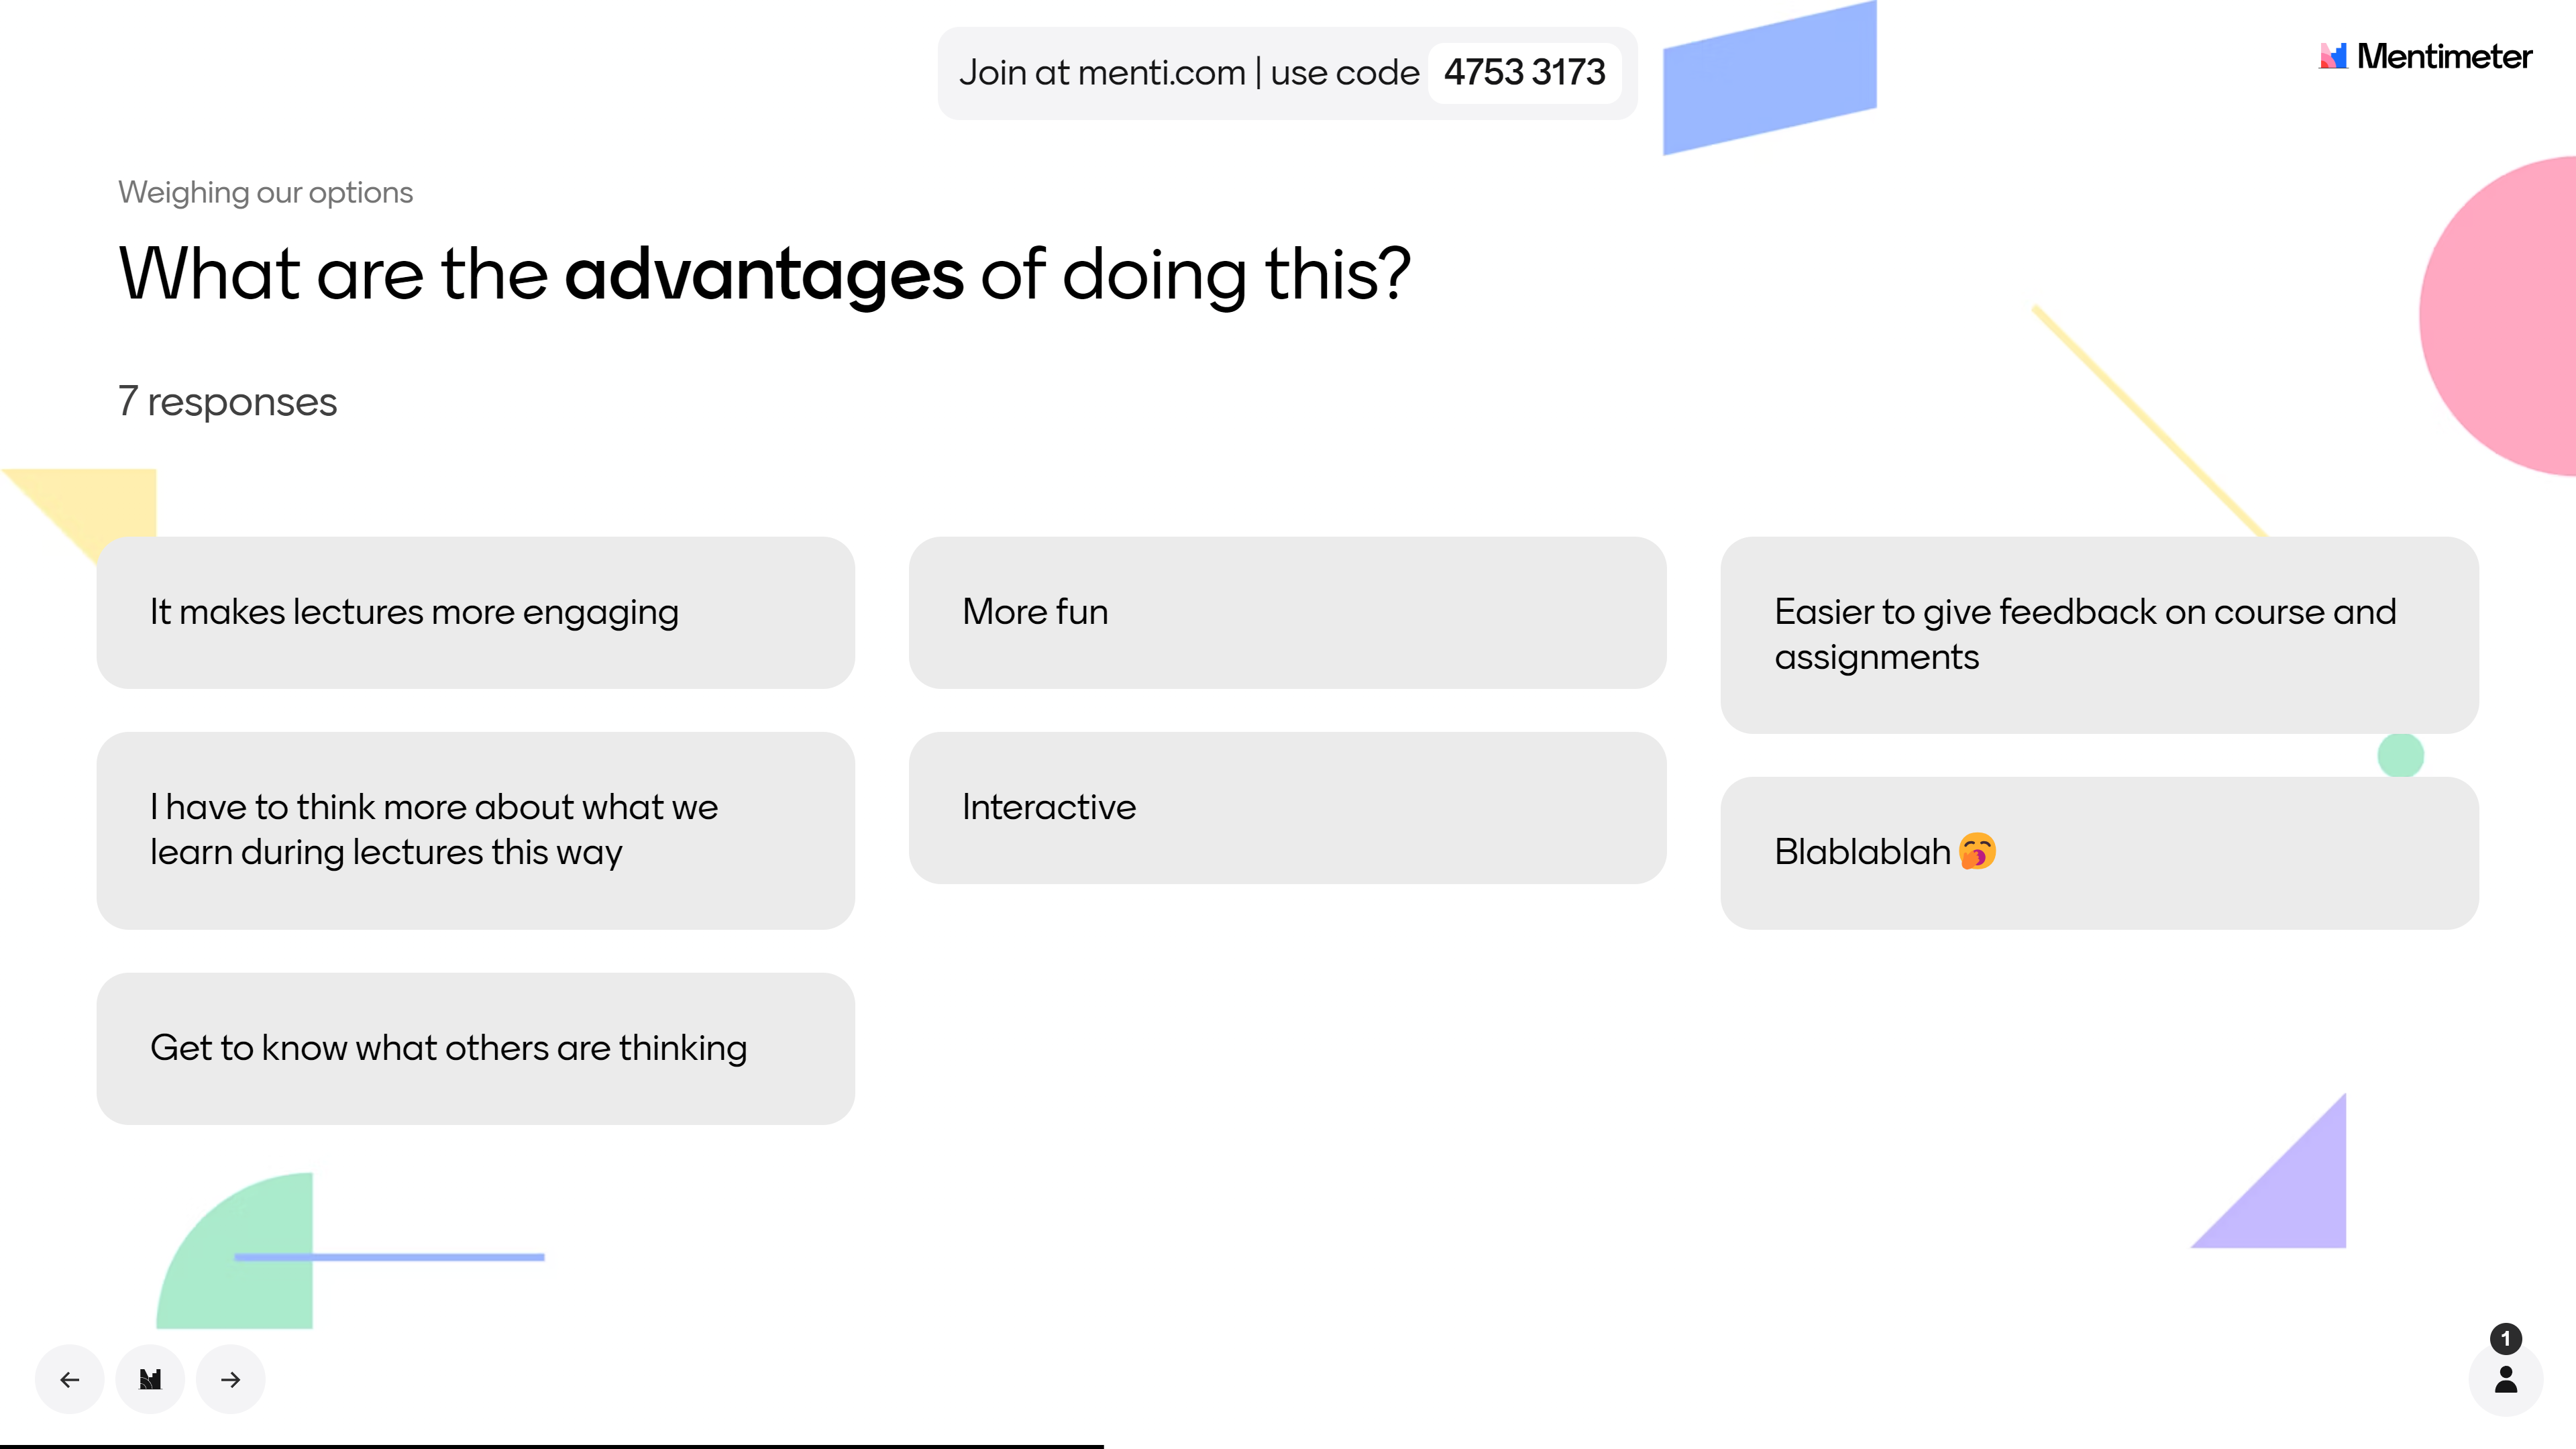
\includegraphics[width=\textwidth]{figures/Mentimeter-host.png}
    \caption{Slide with seven open-text responses as seen by the whole class}
    \label{fig:mentimeterhost}
\end{subfigure}
\hfill
\begin{subfigure}{0.3\textwidth}
    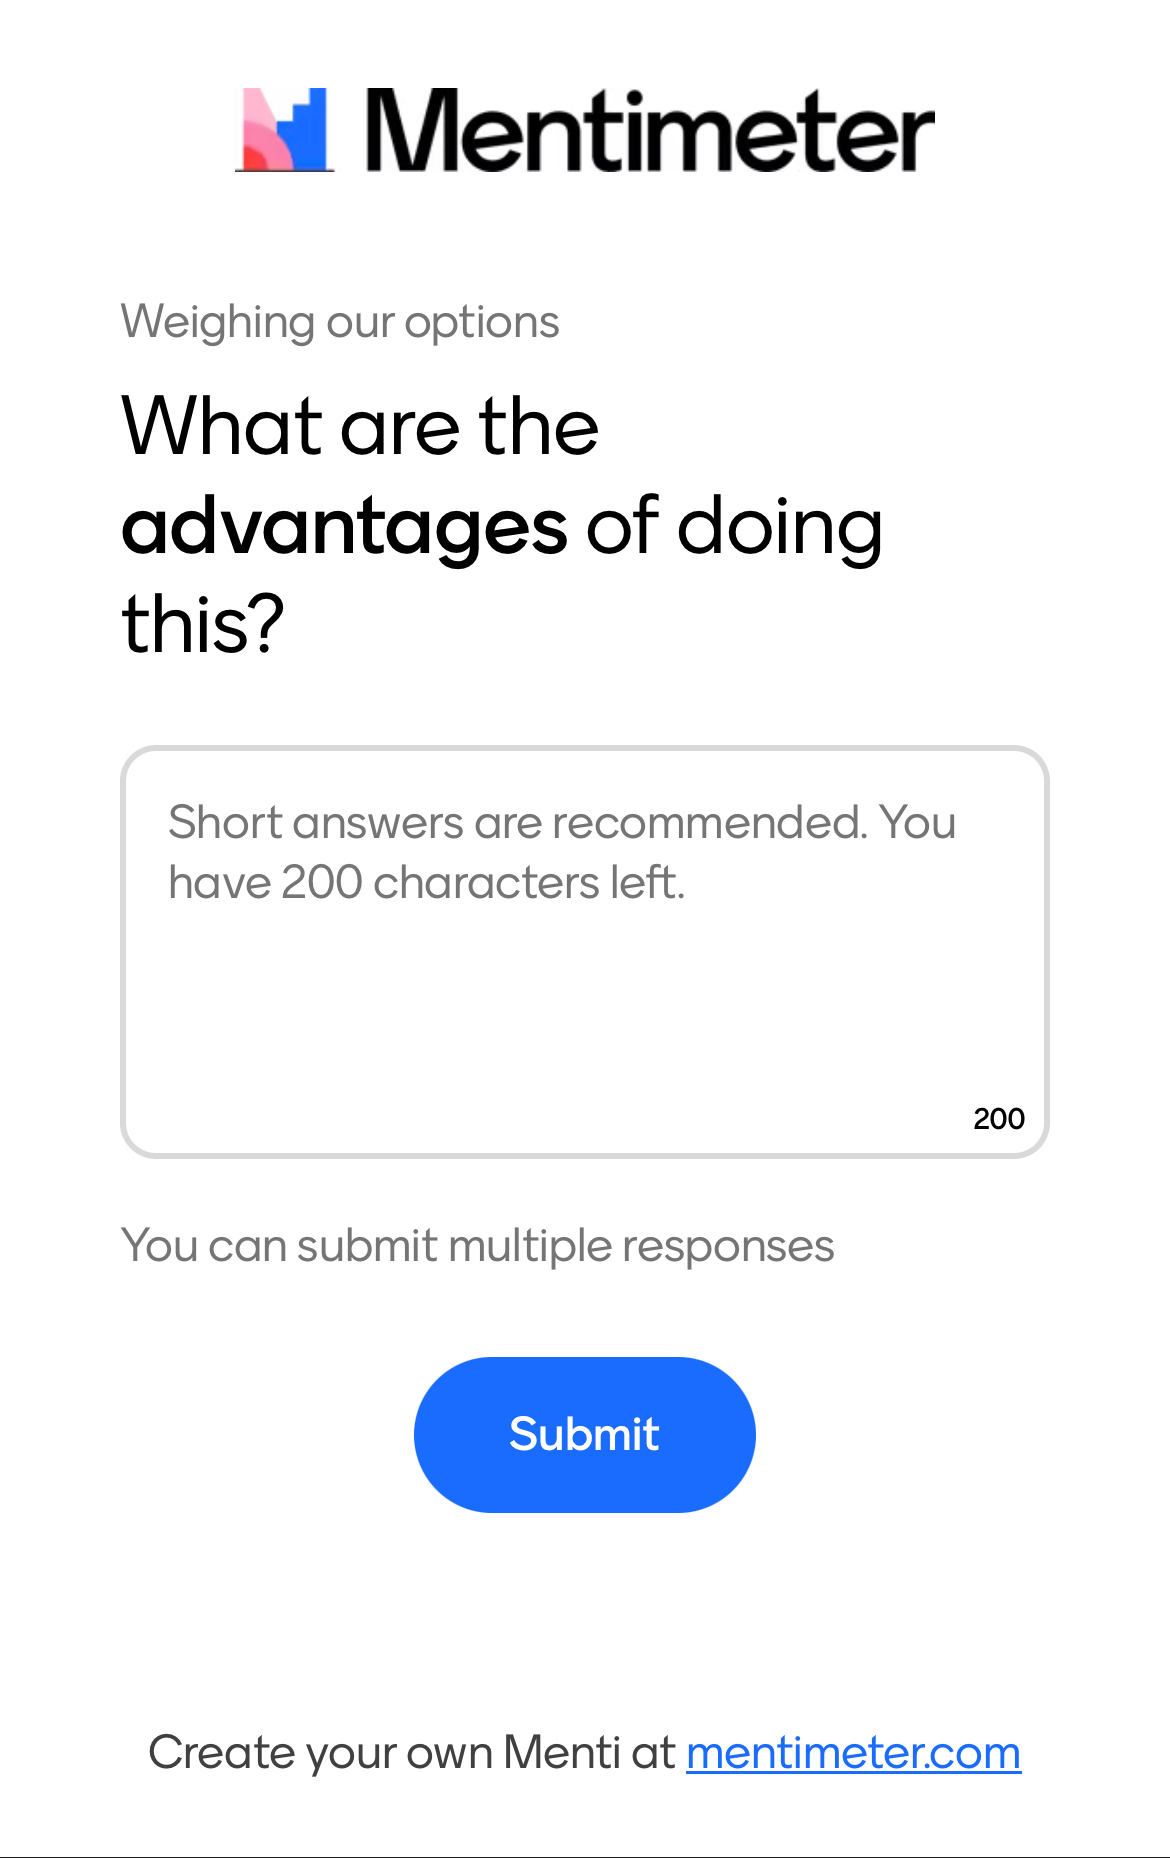
\includegraphics[width=\textwidth]{figures/Mentimeter-client.jpg}
    \caption{Prompt as seen by a student on a phone}
    \label{fig:mentimeterclient}
\end{subfigure}
        
\caption{Screenshots of a slide presented on the Mentimeter website featuring an open-ended question}
\label{fig:mentimeterscreenshots}
\end{figure}

\subsection{Kahoot!}
Kahoot! is described as a learning and engagement platform, and its mission is to ``Make learning awesome'' \cite{kahootAboutKahoot}. Kahoot! uses gamification as the main driver for engagement and features a few different game modes. The ``classic'' mode is the most used. The audience connects to a Kahoot! session from their devices using a pin or QR-code through the Kahoot! app or website. They may then choose a nickname and avatar and will be presented with some multimedia or questions. Answering a question gives users points, with extra points for answering correctly and quickly. On top of this, music, sound effects, a leaderboard and answering streaks contribute to increasing engagement and creating a competitive environment. Similarly to Mentimenter, Kahoot! has various question types. They divide the types into questions for testing knowledge and questions for collecting opinions. We are here only interested in the two types ``Open-ended'' and ``Brainstorm''. These serve to collect opinions and let the audience enter open-text responses of up to 250 and 75 characters, respectively. Figure \ref{fig:kahootsetup} shows a setup for Kahoot! involving a smartphone of the student, the cloud-based servers that process the questions and responses, and the display with the questions and answer alternatives shown to the whole class.

\begin{figure}[h!]
    \centering
    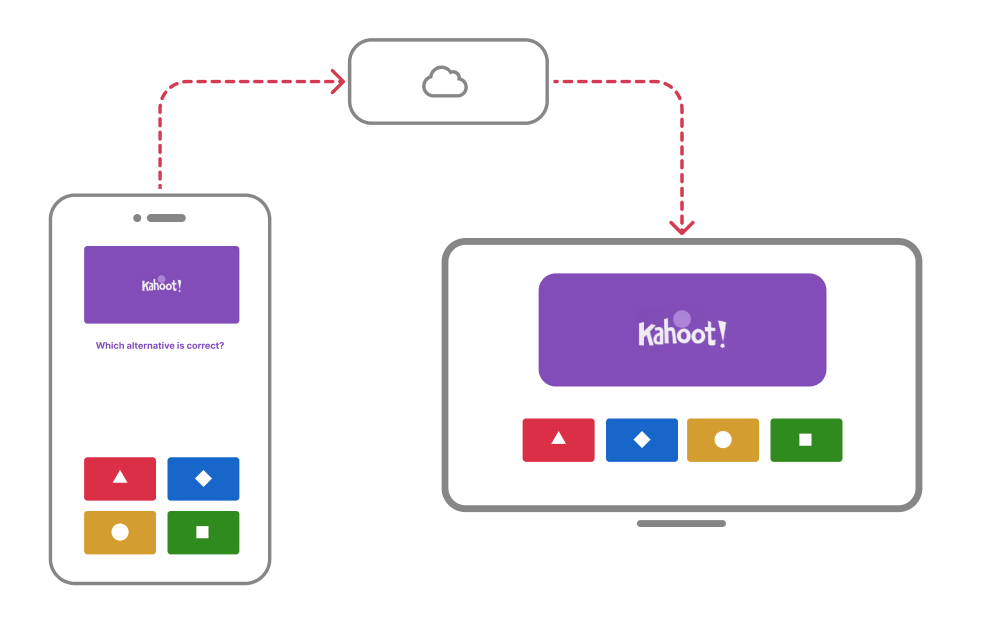
\includegraphics[width=.8\linewidth]{figures/kahoot-illustration.png}
    \caption{A Kahoot setup with phones and a display screen}
    \label{fig:kahootsetup}
\end{figure}

\todo{Include images of Kahoot! GUI}

\section{Challenges with the current systems}
% Also include, positive impacts of our system
% Se 3.5.2 i https://link.springer.com/article/10.1007/s10639-021-10732-8#Sec15 (altså \cite{resyslitrev})
% TODO: Fredrik
\todo{Challenges with the current systems}


\section{Problem of interpreting open-ended questions}
\todo{Large classrooms, actionable insights}
Interpreting written open-ended answers becomes more cumbersome based on the amount of responses. This usually means that such a system is difficult to use for large classes. 

The time it would take for the lecturer to read and comprehend the responses would take too much focus away from the lecture, potentially reducing the efficiency of the lecture. 

A possible solution could be to have a new role, responsible as administrator of the responses, which role is to read and make optimizations for the lecturer while the lecturer is teaching. However this might cause a weird dynamic, as processes in parallell might take focus away from the learning process.

While smaller classes might make it feasible to read through all responses, it might still be difficult to compare or group responses and make actionable insights. 



% Explain AI, NLP, Text-mining, Sentimental Analysis

% Explain how this can extract themes, gauge sentiment, or detect common misconceptions

% Describe challenges of applying NLP to educational data, such as dealing with informal language, typos, or multilingual responses

% Illustrate how AI-driven insights could influence lesson planning or live lecture adjustments, offering concrete examples like identifying misunderstood topics or gaps in student comprehension.

% Discuss how summarization or clustering could help lecturers prioritize feedback on students’ misunderstandings and adapt teaching in real-time.









\begin{comment}
Research projects should always be based on previous research on the same and/or related topics. This should be described as a background to the thesis with adequate bibliographical references. If the material needed is too voluminous to fit nicely in the review part of the introduction, it can be presented in a separate background chapter.
\end{comment}